% ======================================================================================================
% TCC - César Henrique Bernabé
% Capítulo 2 - Referencial Teórico

% 
% ======================================================================================================
\chapter{Referencial Teórico}
\label{sec-referencial}

Este capítulo apresenta os principais conceitos teóricos que fundamentaram a evolução do metamodelo de requisitos do \zanshin e do desenvolvimento da ferramenta \unagi. A seção~\ref{sec-referencial-engenharia-objetivos} aborda a Engenharia de Requisitos Orientada a Objetivos, destacando os principais conceitos dessa área que foram utilizados ao longo deste trabalho. A seção~\ref{sec-referencial-zanshin} apresenta o sistema \zanshin e os detalhes do metamodelo original do \textit{framework}. A seção~\ref{sec-referencial-unagi} apresenta as principais ferramentas que foram utilizadas durante o desenvolvimento do \unagi, como as funcionalidades de Desenvolvimento Orientado a Modelos (\textit{Model Driven Development} ou MDD) do \eclipse, o plugin \sirius, dentre outros.

% ======================================================================================================
% SEÇÃO Engenharia de Requisitos Orientada a Objetivos
% ======================================================================================================

\section{Engenharia de Requisitos Orientada a Objetivos}
\label{sec-referencial-engenharia-objetivos}

% Engenharia de Software
A Egenharia de Software é uma área da Ciência da Computação voltada ao estudo dos processos, métodos, técnicas, ferramentas e ambientes de suporte ao desenvolvimento de software, apoiando-se principalmente nas práticas e aplicações da área de Gerência de Projetos com o objetivo de promover melhor organização, produtividade e qualidade em todo o processo de desenvolvimento de um software ~\cite{falboEngSoft}.

% Engenharia de Requisitos
Dentro da área de Engenharia de Software, destaca-se uma importante subárea, a área de Egenharia de Requisitos de Software, focada no processo de elicitação de requisitos, considerados fatores determinantes no sucesso do desenvolvimento de um software ~\cite{falboEngReq}. Requisitos podem ser entendidos como a definição do que o sistema pode prover, ou também entendidos como o que o sistema é capaz de fazer para atingir um determinado objetivo ~\cite{pfleeger2004engenharia}.

% Objetivos
Devido ao fato de requisitos estarem diretamente ligados aos objetivos do sistema, destaca-se também a \textbf{Engenharia de Requisitos Orientada a Objetivos}, uma parte subárea de Engenharia de Requisitos. Objetivos são parte importante do processo Engenharia de Requisitos, seu propósito é indicar as principais necessidades que justificam a criação de um determinado sistema, demonstrando os casos em que as funcionalidades do mesmo satisfarão as necessidades elicitadas, além de dizer como o sistema deve ser construído para satisfazê-las ~\cite{ross1977structured}. Em uma descrição geral e resumida do processo de identificação de objetivos, pode-se dizer que o potencial software é analisado nos ambientes organizacional, operacional e técnico, onde são assim identificados os problemas de contexto e as oportunidades de solução desses problemas. Então, os objetivos são criados com foco na resolução dos problemas e das oportunidades identificadas. Tendo em mãos os objetivos do sistema devidamente refinados, os requisitos do sistema são então elaborados para que esses objetivos sejam devidamente atendidos. Além de apoiar no processo de modelagem de requisitos, objetivos são usados para apoiar outros propósitos como gerenciamento de conflitos e o processo de verificação ~\cite{van2001goal}. De acordo com ~\cite{van2001goal}, objetivos podem ser reformulados em diferentes níveis de abstração, dependendo do tipo de necessidade que o sistema alvo deve atender, abrangendo desde interesses referentes a estratégias de negócios até conceitos técnicos de atividades, podendo assim referirem-se a requisitos funcionais e não-funcionais.

% Importancia Objetivos
A necessidade de uso de objetivos no processo de modelagem de sistemas de software vem se tornando cada vez mais clara a medida que analistas percebem que:
\begin{itemize}
	\item Objetivos provêm critérios claros de completude dos requisitos do sistema, permitindo também que requisitos desnecessários sejam descartados.
	\item Objetivos facilitam o processo de entendimento dos requisitos por parte dos \textit{stakeholders}.
	\item Melhora a legibilidade de documentos de especificação de requisitos, pois permite que engenheiros possam enxergar com mais clareza as alternativas de desenvolvimento dos requisitos do sistema. Além de facilitar o processo de gerenciamento de conflitos.
	\item Objetivos dirigem parte do processo de elicitação de requisitos, facilitando a identificação de boa parte deles.	
\end{itemize}

% Hardgoal, Softgoal, Quality Constraint e Domain Assumption
Diferentemente dos requisitos, objetivos podem precisar da cooperação entre diferentes tipos de refinamentos para que sejam atendidos de forma suficiente ~\cite{dardenne1993goal}. Em outras palavras, um objetivo diretamente relacionado ao sistema a ser criado torna-se um requisito, enquanto um objetivo sob responsabilidade de um agente do ambiente em que o software será executado torna-se uma Pressuposição de Domínio (ou \textit{Domain Assumptions}) e, nesse caso, são satisfeitos devido a uma regra de negócio ~\cite{van2001goal, van1998managing}. Objetivos funcionais podem ser classificados como objetivos rígidos (\textit{Hard Goals}) e objetivos fracos (\textit{Soft Goals}), estes não possuem critérios claros de satisfação, entretanto são úteis quando deseja-se comparar os melhores refinamentos ao objetivo estudado, enquanto aqueles são objetivos cujo critério de satisfação pode ser atendido de forma técnica ~\cite{dardenne1993goal}. Para que \textit{Soft Goals} tenham um parâmetro claro de satisfabilidade, são adicionados a eles as \textit{Quality Constraints}, critérios que operacionalizam os \textit{Soft Goals}. Por exemplo, um \textit{Soft Goal} ``Baixo Custo'' pode ser refinado na \textit{Quality Constraint} ``Custo deve ser menor que mil reais''. Por fim, ~\cite{jureta2008revisiting} define outro tipo de refinamento para especificar a atendibilidade de um objetivo: as tarefas ou \textit{Taks}, que são os passos a serem tomados para que um determinado objetivo seja cumprido. Em outras palavras, tarefas são definidas por funcionalidades do sistemas que, se executadas com sucesso, são consideradas satisfeitas ~\cite{souza2012requirement}.

% Refinamentos
Objetivos relacionam-se um com o outro através de refinamentos. Segundo ~\cite{dardenne1991goal, dardenne1993goal}, objetivos podem ser refinados usando grafos E/OU (\textit{AND/OR}). O critério de satisfabilidade de objetivos refinados em ``E'' ou ``OU'' segue os conceitos da lógica booleana: refinamentos do tipo ``E'' implicam que para que um objetivo seja considerado satisfeito, todos os sub-objetivos refinados a partir dele devem ser satisfeitos, enquanto refinamentos do tipo ``OU'' relacionam o objetivo principal com um conjunto de alternativas, ou seja, basta que um de seus refinamentos seja atendido para que ele também seja considerado alcançado. Objetivos são refinados até atingirem um level de granularidade em que são refinados apenas por tarefas que podem ser completado com sucesso por um ator (humano ou outro sistema) ~\cite{souza2013awareness}. Refinamentos podem acontecer entre Objetivos e outros Objetivos, \sofgoals, Tarefas e Pressuposições de Domínio.

%Representação Gráfica
Em questões de representação gráfica, os modelos de objetivos discutidos nesse texto são grafos ordenados com as exigências das partes interessadas no topo do modelo e abaixo, objetivos (e tarefas) mais refinados. A simbologia utilizada é baseada na sintaxe de \istar ~\cite{yu20111}. Um exemplo de modelo de objetivos representando um sistema de despacho de ambulâncias é mostrado na Figura ~\ref{figura-acad-simples}.

\begin{figure}[h]
	\centering
	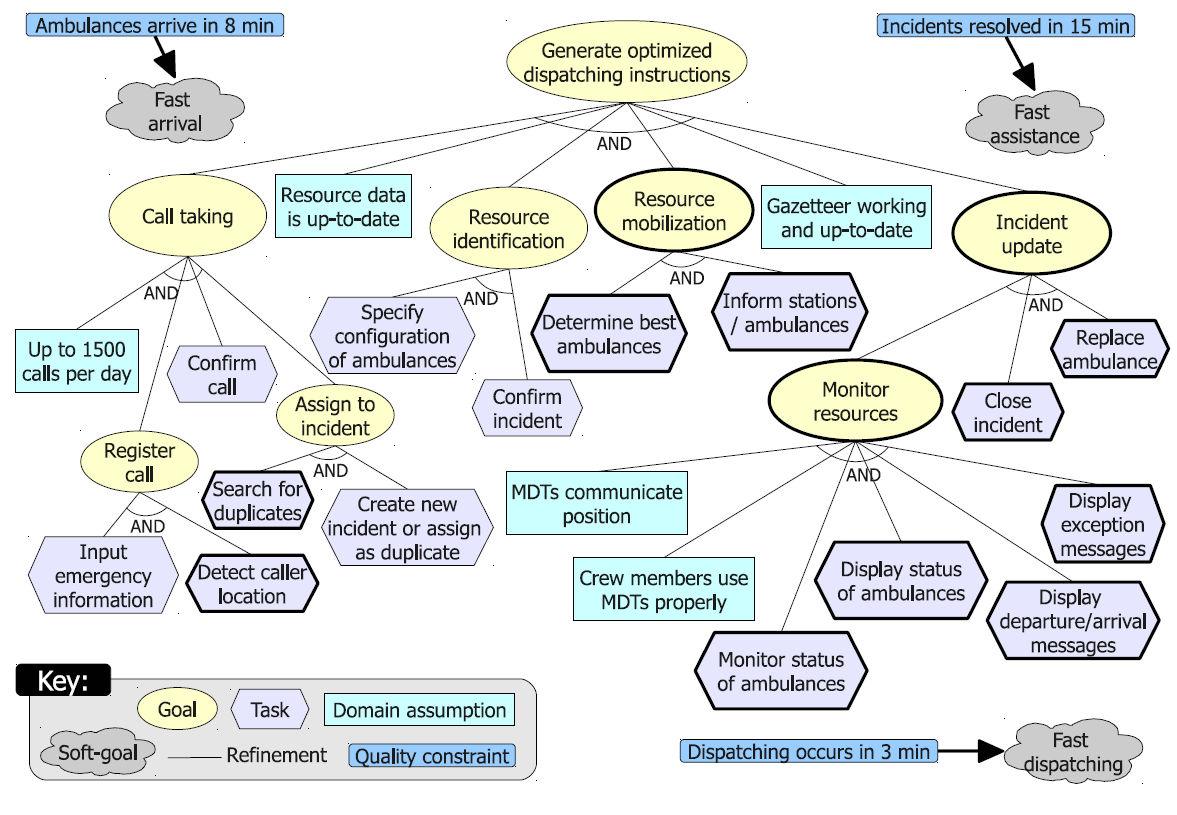
\includegraphics[width=1\textwidth]{figuras/modelos/ACAD-Simples.png}
	\caption{Exemplo de modelos de objetivos ~\cite{tesevitor}}
	\label{figura-acad-simples}
\end{figure}

% ======================================================================================================
% SUBSEÇÃO Modelos de Objetivos em Tempo de Execução
% ======================================================================================================

\subsection{Modelos de Objetivos em Tempo de Execução}
\label{sec-referencial-engenharia-objetivos-runtime}

% Sistemas adaptativos
Muitas vezes os requisitos de um \textit{software} precisam ser modificados durante o ciclo de execução do mesmo. Além disso, durante o processo de especificação as partes interessadas no sistema podem apresentar requisitos condicionais, ou seja, que assumem diferentes configurações dependendo da ocorrência de determinada situação ~\cite{souza2012requirement}. Em outras palavras, há a necessidade de sistemas que possam se automonitorar e, caso necessário, se adaptarem para que seus objetivos continuem sendo satisfeitos ~\cite{dalpiaz2013runtime}. Esse tipo de sistema geralmente é composto por duas partes principais: a primeira sendo o sistema em si, que executa uma tarefa para cumprir um objetivo desejado e a segunda sendo um sistema de monitoramento do primeiro, que envia ao primeiro sistema instruções de modificação de suas configurações para que seus objetivos continuem sendo atendidos ~\cite{souza2013awareness}. 

O sistema de monitoramento é construído fundamentado na premissa de que todo sistema possui um ciclo de retroalimentação (\textit{(feedback loop)}) ~\cite{brun2009engineering}, e assim realizam o processo de adaptação com base nesse ciclo, aplicando controladores de \textit{feedback} que monitoram o comportamento do sistema e injetam estratégias de adaptação ~\cite{souza2013awareness}. O módulo adaptador do sistema verifica, de acordo com as saídas do sistema alvo, se os objetivos internos a esse estão sendo atendidos e, para isso, necessita importar o modelo de objetivos ~\cite{souza2013awareness} enriquecido de elementos que indicam os requisitos a serem observados e as estratégias de adaptação relativas.

Modelos de sistemas adaptativos incluem requisitos autoconscientes, ou seja, requisitos definidos em relação ao sucesso, falha ou qualidade de serviço de outros requisitos ~\cite{souza2013awareness}. Assim, esses requisitos são considerados ``requisitos especiais'' já que sua operacionalização está relacionada a mudança de outros requisitos ~\cite{souza2012requirement}. Ademais, o comportamento do sistema é caracterizado por eventos que ocorrem em tempo de execução e que estão diretamente ligados a instâncias de objetivos ~\cite{dalpiaz2013runtime}. Assim, é importante observar que essa abordagem é considerada orientada a objetivos já que os requisitos mencionados são derivados do refinamento de objetivos elicitados para o sistema.

%Awreqs
Requisitos autoconscientes são divididos em dois tipos principais: Requisitos de Percepção (\textit{Awareness Requirements} ou \awreqs) ~\cite{souza2013awareness} e Requisitos de Evolução (\textit{Evolution Requirements} ou \evoreqs) ~\cite{souza2012requirement}. \awreqs são requisitos que referem-se ao estado de outros requisitos em tempo de execução, representando situações onde as partes interessadas desejam que o sistema se adapte ~\cite{souza2012requirement}. Podem se referir a qualquer tipo de elemento, sejam objetivos, \sofgoals, tarefas e pressuposições de domínio. Além disso, indicam o quão critico um requisito pode ser ao descrever o grau de tolerância a falhas do mesmo ~\cite{souza2012requirement}. Antes da execução de um sistema, os requisitos estão em estado ``não decidido'' (\textit{undecided}), e então pode assumir os estados ``Sucesso'' (\textit{Succeeded}), ``Falha'' (\textit{Failed}), e no caso de objetivos e tarefas, ``Cancelado'' (\textit{Canceled}) ~\cite{souza2013awareness}. É facilmente notável que o processo de elicitação de requisitos de percepção só acontece depois que o modelo de objetivos é levantado, e assim como o processo de construção de objetivos, \awreqs devem ser sistematicamente criados.

%Evoreqs
\evoreqs são requisitos que modificam o espaço de comportamento do sistema, permitindo que novas alternativas de requisitos sejam usadas, baseando-se em um conjunto pré-definido de etapas de evolução para os requisitos monitorados ~\cite{souza2012requirement}. Isto é, \evoreqs são requisitos que especificam uma série de operações primárias em relação a outros  requisitos diante de determinadas situações, dizendo ao sistema como adaptar-se \cite{souza2012requirement}. Por exemplo, adicionar ou remover um objetivo, modificar o estado de um objetivo (em nível de instância), desfazer as ações de uma execução que resultou em falha, entre outras ~\cite{souza2013requirements}.

Em suma, \awreqs especificam quando um determinado objetivo precisa de mudanças para continuar a ser atendido, enquanto \evoreqs especificam como executar tais mudanças. A seguir, o modelo de exemplo apresentado na seção \ref{sec-referencial-engenharia-objetivos} é novamente apresentado, porém com novos requisitos de adaptação que são devidamente discutidos na próxima sessão.

% ======================================================================================================
% SUBSEÇÃO Exemplo de Caso de Uso
% ======================================================================================================
\subsection{Exemplo de Modelagem de Caso de Uso}
\label{sec-referencial-engenharia-objetivos-exemplo}

Na Figura \ref{figura-acad-completo} é apresentado o modelo completo do sistema de despacho de ambulâncias (\textit{Adaptive Computer-aided	Ambulance Dispatch} ou \textit{A-CAD}), nele observa-se o objetivo principal "Gerar Instruções de Despacho Otimizadas", representado por uma oval, que é imediatamente refinado em outros objetivos e em uma pressuposição de domínio, representada por retângulos, o refinamento entre o objetivo raiz e seus filhos imediatos é do tipo ``E'', portanto, para que o objetivo principal seja considerado satisfeito, todos as suas decomposições precisam ser satisfeitas. Então, verifica-se que o primeiro nível de refinamento do objetivo principal é composto de:

\begin{itemize}
	\item Objetivo: ``Gerenciar Chamadas''
	\item Objetivo: ``Identificação de Recursos''
	\item Objetivo: ``Mobilização de Recursos''
	\item Objetivo: ``Obtenção de Mapas''
	\item Pressuposição de Domínio: ``Dados sobre recursos está sempre atualizado''
\end{itemize}

O processo de refinamento do modelo então segue até que todos os objetivos sejam completamente refinados em tarefas ou pressuposições de domínio. \sofgoals são representados por nuvens e refinados em critérios de operacionalização (os \textit{Quality Constraints}) representados por retângulos com cantos arredondados. Para exemplificar: o \sofgoal ``Chegada Rápida''é operacionalizado por ``Ambulâncias chegam em oito minutos'', assim, tem-se um critério claro de satisfação para um objetivo que antes possuía diversos tipos de interpretação, porém agora, sabemos que uma ambulância chega rapidamente se consegue estar no local do acidente em menos de oito minutos a partir da chamada.

Os requisitos de percepção são representados por um círculo oco. O modelo da \ref{figura-acad-completo} possui ao todo 16 tipos de \awreqs. Por exemplo, o \awreq identificado por ``AR15'', indica que o objetivo ``Registrar Chamados'' deve ``Nunca falhar''. Os \evoreqs referentes a cada um dos \awreqs não são representados nesse modelo, e devem ser especificados em forma de sequencia de operações sobre os elementos do modelo de objetivos (essa escolha visa facilitar a legibilidade do modelo). Além dos \evoreqs, são especificados também os parâmetros de controle (\textit{control parameters}), representados por losangos, que indicam parâmetros do sistema que podem ser reconfigurados para adaptação. As formas de representação estão resumidas na Figura \ref{figura-elementos-gore-eca}.

Sobre os \evoreqs do AR15, podemos definir seus respectivos Requisitos de Evolução. Primeiramente, se o objetivo vir a falhar, define-se a primeira estratégia de adaptação como ``Tentar Novamente em 5 segundos no máximo uma vez'' (\texttt{RetryStrategy(5000);}), caso falhe mais do que uma vez, aplica-se outra estratégia ``Diminuir Condições ao Desabilitar Filho'' (\texttt{RelaxDisableChild(T_DetectCaller);}), que desativa o requisito ``Detectar Localização da Ligação'', também aplicado no máximo uma vez. Essas decisões são sumarizadas na tabela \ref{tabela-evoreqs-ar15}.

\begin{table}[]
	\centering
	\caption{Tabela de especificação das estratégias de adaptação de AR15.}
	\label{tabela-evoreqs-ar15}
	\begin{tabular}{lll}
		AR15 & NeverFail(G\_RegCall) & \begin{tabular}[c]{@{}l@{}}1. Retry(5000)\\ 2. RelaxDisableChild(T DetectCaller)\end{tabular}
	\end{tabular}
\end{table}

\begin{figure}[h]
	\centering
	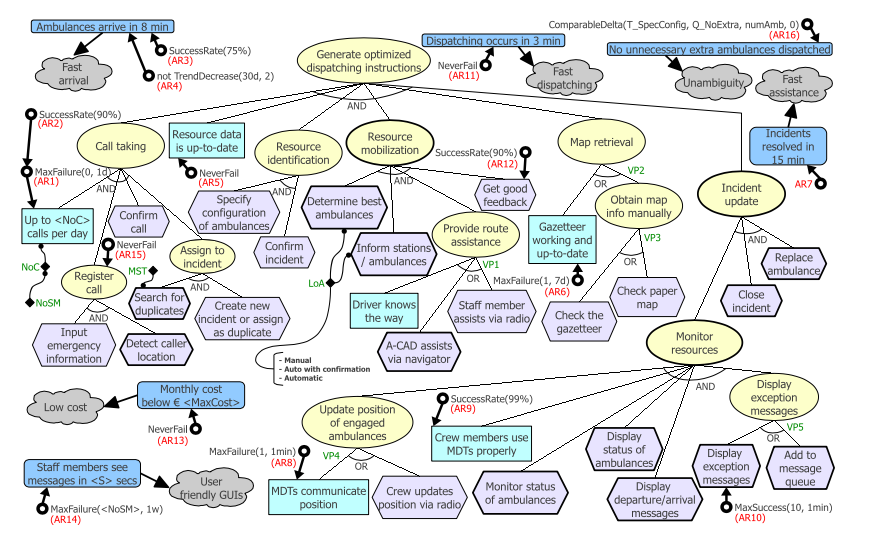
\includegraphics[width=1\textwidth]{figuras/modelos/ACAD-Completo.png}
	\caption{Exemplo de modelos de objetivos de um sistema de despacho de ambulâncias ~\cite{tesevitor}}
	\label{figura-acad-completo}
\end{figure}

\begin{figure}[h]
	\centering
	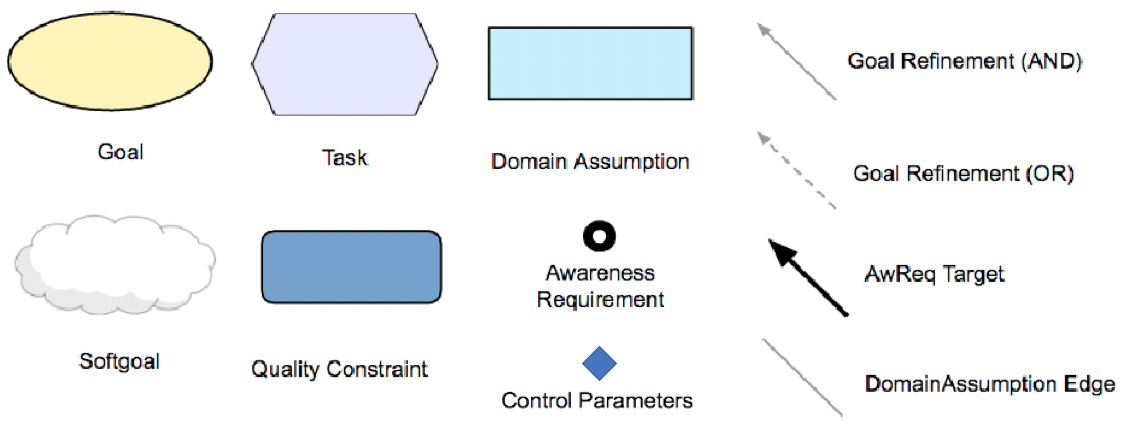
\includegraphics[width=1\textwidth]{figuras/modelos/Elementos-GORE.png}
	\caption{Representação gráfica de elementos de \gore}
	\label{figura-elementos-gore-eca}
\end{figure}


% ======================================================================================================
% SEÇÃO Zanshin
% ======================================================================================================

\section{Zanshin}
\label{sec-referencial-zanshin}

Apresentado por ~\cite{tesevitor} e baseado em várias das premissas discutidas até aqui, \zanshin é um \textit{framework} que utiliza de ciclos de retro-alimentação para monitorar requisitos e enviar estratégias de adaptação com base em informações de modelos de requisitos orientados a objetivos enriquecidos com elementos como os \awreqs e os \evoreqs. 

% ======================================================================================================
% SUBSEÇÃO Zanshin: Monitoramento
% ======================================================================================================
\subsection{Monitoramento}
\label{sec-referencial-zanshin-monitoramento}

Em tempo de execução, os elementos do modelo de objetivos são representados por classes e instanciados cada vez que o usuário (ou sistema) busca atingir um objetivo, e então o sistema passa a enviar mensagens a essas instâncias quando detectar falhas. Percebe-se assim, que objetivos e pressuposições de domínio não são tratadas como invariantes que devem sempre ser atingidas, já que o sistema pode falhar ao tentar atingir seus objetivos iniciais, e assim o sistema de adaptação lidará com essas falhas e tomará medidas para que os objetivos voltem a ser satisfeitos ~\cite{souza2013requirements}.

Assim como o monitoramento de objetivos através do \textit{Feddback Loop}, o \zanshin também monitora Parâmetros (\textit{Parameters}) que podem ser definidos em dois tipos. Pontos de Variação (ou \textit{Variation Points}), que representam refinamentos do tipo ``OU'' (\textit{OR}). Por exemplo, o VP4 do modelo de objetivos do sistema A-CAD (Figura \ref{figura-acad-completo}) que refere-se ao objetivo ``Atualizar posição de ambulâncias em uso'' especifica que atualizações de posição das ambulâncias podem ser obtidas automaticamente ou via rádio. Variáveis de Controle (ou \textit{Control Variables}) são abstrações referentes a pontos de variação repetitivos ou usados em grande escala, como por exemplo a variável MST (``Tempo de Busca Mínimo'' ou \textit{Minimum Search Time}), que refere-se a tarefa ``Procurar por (incidentes) duplicados''.

%TODO: acho que aqui pode começar a explicar os modulos de monitoramento e adaptação, e aproveitara pra ja mostrar o metamodelo de classes original do zanshin, sem citar o meu novo lindo.

% ======================================================================================================
% SUBSEÇÃO DESENVOLVIMENTO ORIENTADO A MODELOS
% ======================================================================================================

%TODO: Falar de MDD de forma geral, com leve foco no Eclipse Modeling Tools, e entao introduzir o sirius.

\section{Desenvolvimento Orientado a Modelos}

\subsection{Sirius}

